% ============================================================
% Chapter 2: Statistical Model and Sampling
% ============================================================
\chapter{Statistical Model and Sampling}
\label{ch:model}

\begin{center}
\textit{``All models are wrong, some are useful.''} --- George Box
\end{center}

\section{Motivating Example}

A pharmaceutical lab tests a new drug. Out of $n=100$ patients, 68 recover. Is the drug effective? To answer, we need a \emph{model}: assume each patient recovers independently with probability $p$. The 100 results form a \textbf{random sample} from $\mathrm{Bernoulli}(p)$.

\section{Statistical Model}

\begin{definition}[Statistical Model]
\index{statistical model}
A \textbf{statistical model} is a triple $(\mathcal{X}, \mathcal{A}, \mathcal{P})$ where:
\begin{itemize}
\item $\mathcal{X}$ is the \textbf{sample space},
\item $\mathcal{A}$ is a $\sigma$-algebra on $\mathcal{X}$,
\item $\mathcal{P} = \{P_\theta : \theta\in\Theta\}$ is a family of probability distributions indexed by $\theta\in\Theta$.
\end{itemize}
\end{definition}

\begin{definition}[Parametric vs.\ Nonparametric]
\index{parametric model}
\begin{itemize}
\item \textbf{Parametric}: $\Theta\subseteq\R^d$ for finite $d$.
\item \textbf{Nonparametric}: $\Theta$ is infinite-dimensional.
\item \textbf{Semiparametric}: parametric + nonparametric components.
\end{itemize}
\end{definition}

\begin{definition}[Identifiability]
\index{identifiability}
The model is \textbf{identifiable} if $P_{\theta_1}=P_{\theta_2}\implies\theta_1=\theta_2$.
\end{definition}

\section{Random Sample}

\begin{definition}[Random Sample]
\index{random sample}
A \textbf{random sample} of size $n$ from $P_\theta$ is $(X_1,\ldots,X_n)$ where the $X_i$ are \textbf{independent and identically distributed} (i.i.d.) with distribution $P_\theta$. We write $X_1,\ldots,X_n \iid P_\theta$.
\end{definition}

\section{Statistics and Sampling Distributions}

\begin{definition}[Statistic]
\index{statistic}
A \textbf{statistic} is a measurable function $T=T(X_1,\ldots,X_n)$ that does \emph{not} depend on $\theta$.
\end{definition}

\begin{definition}[Sufficient Statistic]
\index{sufficient statistic}
$T$ is \textbf{sufficient} for $\theta$ if the conditional distribution of $(X_1,\ldots,X_n)$ given $T$ does not depend on $\theta$.
\end{definition}

\begin{theorem}[Fisher--Neyman Factorization]
\index{Fisher--Neyman}
$T(\mathbf{X})$ is sufficient for $\theta$ if and only if:
\[
f(\mathbf{x};\theta) = g(T(\mathbf{x}),\theta)\cdot h(\mathbf{x}).
\]
\end{theorem}

\begin{proof}
\textit{(Discrete case.)} If $T$ is sufficient, set $g(t,\theta)=P_\theta(T=t)$ and $h(\mathbf{x})=P(\mathbf{X}=\mathbf{x}\mid T=T(\mathbf{x}))$. Conversely, if the factorization holds:
\[
P_\theta(\mathbf{X}=\mathbf{x}\mid T=t) = \frac{h(\mathbf{x})}{\sum_{\mathbf{y}:T(\mathbf{y})=t} h(\mathbf{y})},
\]
which does not depend on $\theta$.
\end{proof}

\section{Key Sampling Results}

\begin{theorem}[Mean and Variance of $\xbar$]
If $X_1,\ldots,X_n \iid$ with $\E[X_i]=\mu$, $\Var(X_i)=\sigma^2$: $\E[\xbar]=\mu$, $\Var(\xbar)=\sigma^2/n$.
\end{theorem}

\begin{theorem}[Law of Large Numbers]
\index{law of large numbers}
$\xbar \xrightarrow{\Prob} \mu$ (weak) and $\xbar \xrightarrow{\text{a.s.}} \mu$ (strong) as $n\to\infty$.
\end{theorem}

\begin{theorem}[Central Limit Theorem (CLT)]
\index{central limit theorem}
\label{thm:clt}
If $\E[X_i]=\mu$ and $0<\Var(X_i)=\sigma^2<\infty$:
\[
\frac{\sqrt{n}(\xbar-\mu)}{\sigma} \xrightarrow{\mathcal{L}} \mathcal{N}(0,1).
\]
\end{theorem}

\begin{intuition}
The CLT explains the ubiquity of the normal distribution: whenever a quantity results from the \textbf{sum of many small independent effects}, it is approximately Gaussian.
\end{intuition}

\begin{center}
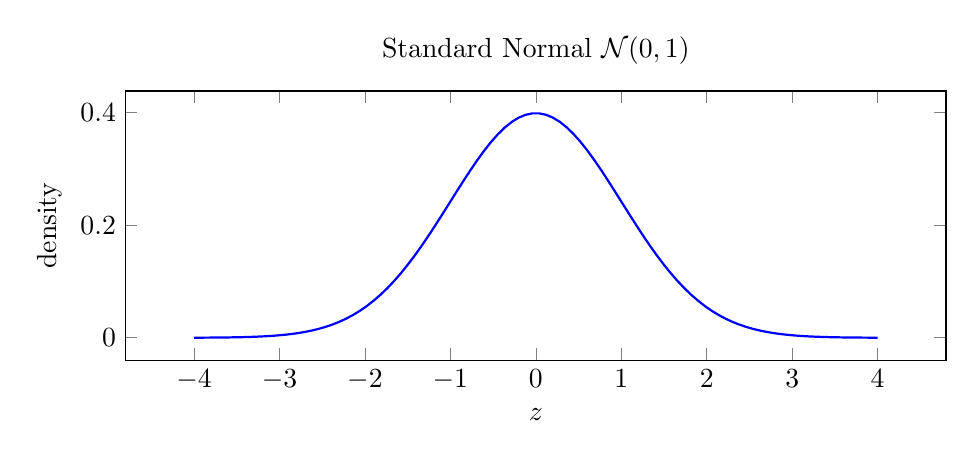
\begin{tikzpicture}
\begin{axis}[width=12cm, height=5cm, domain=-4:4, samples=100, xlabel={$z$}, ylabel={density}, title={Standard Normal $\mathcal{N}(0,1)$}]
\addplot[thick,blue] {exp(-x^2/2)/sqrt(2*pi)};
\end{axis}
\end{tikzpicture}
\end{center}

\section{Distribution of the Sample Variance}

\begin{theorem}[Distribution of $S^2$ under Normality]
\label{thm:s2-dist}
If $X_1,\ldots,X_n\iid\mathcal{N}(\mu,\sigma^2)$:
\begin{enumerate}
\item $\xbar$ and $S^2$ are independent (Cochran's theorem),
\item $(n-1)S^2/\sigma^2\sim\chi^2(n-1)$,
\item $(\xbar-\mu)/(S/\sqrt{n})\sim t(n-1)$.
\end{enumerate}
\end{theorem}

\begin{theorem}[Glivenko--Cantelli]
\index{Glivenko--Cantelli}
$\sup_{x}|\hat{F}_n(x)-F(x)| \xrightarrow{\text{a.s.}} 0$.
\end{theorem}

\section{Python Implementation}

\begin{python}
\begin{minted}{python}
import numpy as np
import matplotlib.pyplot as plt
from scipy import stats

np.random.seed(42)
n_values = [1, 2, 5, 30]
fig, axes = plt.subplots(1, 4, figsize=(16, 3.5))
for ax, n in zip(axes, n_values):
    means = [np.mean(np.random.exponential(1, n)) for _ in range(10000)]
    ax.hist(means, bins=40, density=True, alpha=0.7, edgecolor='black')
    ax.set_title(f"n = {n}")
    if n >= 5:
        x = np.linspace(min(means), max(means), 100)
        ax.plot(x, stats.norm.pdf(x, 1, 1/np.sqrt(n)), 'r-', lw=2)
plt.suptitle("CLT: means of exponential samples")
plt.tight_layout()
plt.savefig("ch02_clt.pdf")
plt.show()
\end{minted}
\end{python}

\section{Exercises}

\begin{exercise}[$\star$]
Sample of size $n=25$ from $\mathcal{N}(10,4)$. Compute $\E[\xbar]$, $\Var(\xbar)$, and $\Prob(|\xbar-10|>0.5)$.
\end{exercise}

\begin{exercise}[$\star$]
Generate 10,000 sample means of size $n=30$ from $\mathrm{Unif}([0,1])$. Verify graphically that the CLT holds.
\end{exercise}

\begin{exercise}[$\star\star$ -- Sufficiency]
Show that $T=\sum X_i$ is sufficient for $\lambda$ when $X_i\iid\mathrm{Pois}(\lambda)$.
\end{exercise}

\begin{exercise}[$\star\star$ -- CLT proof via characteristic functions]
Prove the CLT using the expansion $\varphi(t)=1-t^2/2+o(t^2)$.
\end{exercise}

\begin{exercise}[$\star\star\star$ -- Project: Monte Carlo convergence study]
Study CLT convergence speed for exponential, Bernoulli, uniform, and Cauchy parent distributions.
\end{exercise}

\begin{keyformulas}
\begin{align*}
\E[\xbar] &= \mu & \Var(\xbar) &= \sigma^2/n \\
\frac{\sqrt{n}(\xbar-\mu)}{\sigma} &\xrightarrow{\mathcal{L}} \mathcal{N}(0,1) &
\frac{(n-1)S^2}{\sigma^2} &\sim \chi^2(n-1) \\
\frac{\xbar-\mu}{S/\sqrt{n}} &\sim t(n-1) &
\sup_x|\hat{F}_n-F| &\xrightarrow{\text{a.s.}} 0
\end{align*}
Fisher--Neyman: $f(\mathbf{x};\theta) = g(T(\mathbf{x}),\theta)\cdot h(\mathbf{x}) \iff T$ sufficient.
\end{keyformulas}
